\chapter{Algorithm and Implementation}
In this chapter, we'll look into the algorithm overview and the corresponding code implementation.

\section{Pre-Computing Optical Depth}
The first step is to pre-compute the optical depth using Equation 2.2: $\tau(A, B) = \int_{A}^{B}\beta(P)\cdot ds$ for each ray to the boundary of a certain particle. The author assumed that the camera will always stay outside the volume. Then, the goal of this step is to calculate the optical depth integral for all possible camera positions and orientations.

\begin{figure}[htp]
\begin{center}
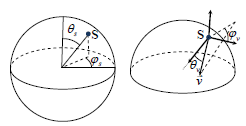
\includegraphics[scale=1.0]{images/startandview.png}
\caption{Four angels to describe a ray}
\label{f8}
\end{center}
\end{figure}

\subsection{The Design}
To describe a ray, we need 4 angles, 2 angles describing the start point on the particle sphere, and 2 angles describing the view direction. Because of the 4 parameters, a 4D look-up table is necessary. As shown in the figure above, $\varphi_S\in[0, 2\pi]$ and $\theta_S\in[0, \pi]$ are used to specify the start point of the ray. While $\varphi_v\in[0, 2\pi]$ and $\theta_v\in[0, \frac{\pi}{2}]$ are used to specify the direction of the ray.\\\\\\

\begin{figure}[htp]
\begin{center}
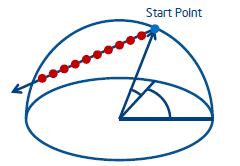
\includegraphics[scale=1.0]{images/opticaldepthintegration.png}
\caption{Numerically integrate the optical depth of a ray}
\label{f9}
\end{center}
\end{figure}

Then we use Equation 2.2: $\tau(A, B) = \int_{A}^{B}\beta(P)\cdot ds$ to accumulate the optical depth of a ray. Now, here is the interesting part of how to retrieve the extinction coefficient $\beta(P)$. The author used 4D look-tables which contains several 3D noises to get the extinction coefficient. The figure below shows one typical noise texture.

\begin{figure}[htp]
\begin{center}
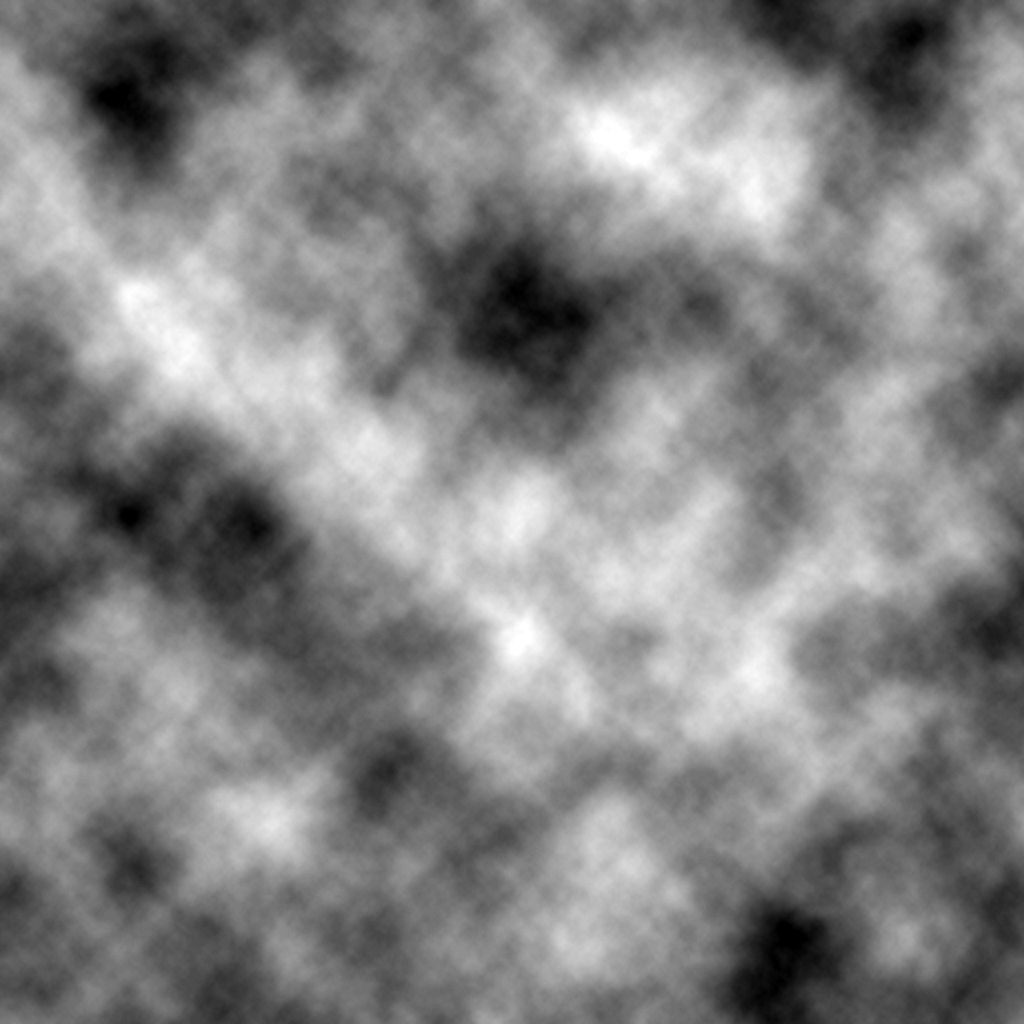
\includegraphics[scale=0.15]{images/Noise.png}
\caption{A typical noise texture}
\label{f10}
\end{center}
\end{figure}

\subsection{The Implementation}
After carefully explaining the design of the first step, let's have a look at how the actual related function in the shader looks like. Please note that the rendering API is \textbf{DirectX}, hence the shader is written in \textbf{HLSL}.\\\\
\begin{lstlisting}
// This shader computes level 0 of the maximum density mip map
float2 PrecomputeOpticalDepthPS(SScreenSizeQuadVSOutput In) : SV_Target
{
    float3 f3NormalizedStartPos, f3RayDir;
    OpticalDepthLUTCoordsToWorldParams( float4(ProjToUV(In.m_f2PosPS), g_GlobalCloudAttribs.f4Parameter.xy), f3NormalizedStartPos, f3RayDir );
    
    // Intersect view ray with the unit sphere:
    float2 f2RayIsecs;
    // f3NormalizedStartPos  is located exactly on the surface; slightly move start pos inside the sphere
    // to avoid precision issues
    GetRaySphereIntersection(f3NormalizedStartPos + f3RayDir*1e-4, f3RayDir, 0, 1.f, f2RayIsecs);
    
    if( f2RayIsecs.x > f2RayIsecs.y )
        return 0;

    float3 f3EndPos = f3NormalizedStartPos + f3RayDir * f2RayIsecs.y;
    float fNumSteps = NUM_INTEGRATION_STEPS;
    float3 f3Step = (f3EndPos - f3NormalizedStartPos) / fNumSteps;
    float fTotalDensity = 0;
    float fDistToFirstMatter = -1;
    for(float fStepNum=0.5; fStepNum < fNumSteps; ++fStepNum)
    {
        float3 f3CurrPos = f3NormalizedStartPos + f3Step * fStepNum;
        
        float fDistToCenter = length(f3CurrPos);
        float fMetabolDensity = GetMetabolDensity(fDistToCenter);
        float fDensity = 1;
#if DENSITY_GENERATION_METHOD == 0
        fDensity = saturate( 1.0*saturate(fMetabolDensity) + 1*pow(fMetabolDensity,0.5)*(GetRandomDensity(f3CurrPos, 0.15, 4, 0.7 )) );
#elif DENSITY_GENERATION_METHOD == 1
        fDensity = 1.0*saturate(fMetabolDensity) + 1.0*pow(fMetabolDensity,0.5)*(GetRandomDensity(f3CurrPos, 0.1,4,0.8)) > 0.1 ? 1 : 0;
#elif DENSITY_GENERATION_METHOD == 2
        fDensity = GetPyroSphereDensity(f3CurrPos);
#endif

        if( fDensity > 0.05 && fDistToFirstMatter < 0 )
            fDistToFirstMatter = fStepNum / fNumSteps;
       
        fTotalDensity += fDensity;
    }
    if( fDistToFirstMatter < 0 ) fDistToFirstMatter = 1;
    return float2(fTotalDensity / fNumSteps, fDistToFirstMatter);
}
\end{lstlisting}

The integration function is \textbf{PrecomputeOpticalDepthPS}. Firstly, it decomposes the given projection position and the 4 angle parameters from inhomogeneous coordinates into 2 vec3 positions, the first one \textbf{f3NormalizedStartPos} describes the start position of the ray, the second one \textbf{f3RayDir} describes the ray direction. Then the intersecting view ray inside the unit sphere is calculated. Since the start position is just on the surface of the sphere, in order to avoid precision issues, the author moved the start position slightly into the sphere by the amount of \textbf{f3RayDir*1e-4}. Then the integration is done inside the \textbf{for loop}. \textbf{DENSITY\_GENERATION\_METHOD} is defined as: 0 represents radial fall-off + 3D noise, 1 represents 3D noise + thresholding, 2 represents pyroclastic style.
\textbf{fDensity} is the current density of this step. Finally, the total density \textbf{fTotalDensity} for a ray is accumulated.


\section{Pre-Computing Scattering}
